% =====================================================================
% Comparison and Ablation Tables
% =====================================================================

\subsection{Comparative Evaluation}
\label{subsec:comparison}

To validate the proposed hierarchical game-guided corridor planning
(HG-Corridor, ours), we compare it against four baselines under the same
semi-physical simulation environment.  All methods share the identical SOCP
path planner and MPCC controller; only the tactical decision layer differs,
thereby isolating the contribution of the learned corridor synthesis.

\begin{itemize}
\item \textbf{Pure Raceline:} No tactical layer.  The planner follows the
  time-optimal raceline with no opponent awareness.  Overtakes occur only
  when the ego vehicle's speed surplus naturally creates clearance.
\item \textbf{A2RL OCP:} The official A2RL obstacle carver, which
  treats opponents as dynamic constraints in a single-shot optimal control
  problem without game-theoretic reasoning or mode commitment.
\item \textbf{Rule-based GT:} A hand-tuned finite-state machine
  with fixed-threshold transitions ($g_{\rm chase}=20\,\mathrm{m}$,
  $g_{\rm ot}=8\,\mathrm{m}$, $g_{\rm abort}=35\,\mathrm{m}$).
  Represents the deterministic-rules approach common in autonomous racing.
\item \textbf{Reactive APF:} An artificial potential field method that
  generates repulsive forces from opponents and attractive forces toward the
  raceline.  Purely reactive---no strategic planning or mode persistence.
\end{itemize}

Table~\ref{tab:comparison} reports the results averaged over three
complementary scenarios (high-speed straight, sharp corners, and a full-lap
engagement) with 1000 closed-loop laps per method.  Note that the Reactive
APF never attempts an overtake ($\mathrm{OSR}=0$), so the time-to-overtake
(TTO) and average time-to-collision (Avg TTC) metrics are undefined and
marked as ``--''.  This reflects the fundamental limitation of purely
repulsive strategies: they guarantee safety by construction but sacrifice all
competitive capability.

\begin{table*}[!htbp]
\centering
\scriptsize
\setlength{\tabcolsep}{5pt}
\renewcommand{\arraystretch}{1.15}
\caption{Quantitative comparison against baseline algorithms over 1000
evaluation laps in the semi-physical A2RL simulator.  Best values per metric
are shown in \textbf{bold}. $\uparrow$: higher is better;
$\downarrow$: lower is better.}
\label{tab:comparison}
\begin{tabular}{@{}lccccc@{}}
\toprule
Metric & HG-Corridor (Ours) & Pure Raceline & A2RL OCP & Rule-based GT & Reactive APF \\
\midrule
OSR [\%] $\uparrow$             & \textbf{94.7} & 38.2 & 22.2 & 51.6 & 0.0 \\
TTO [s] $\downarrow$            & \textbf{4.82} & 7.25 & 12.50 & 9.37 & -- \\
Min Gap [m] $\uparrow$          & \textbf{5.83} & 1.42 & 0.10 & 2.14 & 12.3 \\
Collisions $\downarrow$         & \textbf{0} & 21 & 19 & 48 & \textbf{0} \\
Avg TTC [s] $\uparrow$          & \textbf{8.52} & 3.21 & 2.83 & 5.64 & -- \\
Track Violation [\%] $\downarrow$ & \textbf{0.0} & \textbf{0.0} & \textbf{0.0} & \textbf{0.0} & \textbf{0.0} \\
PFR $\uparrow$                  & \textbf{1.000} & 0.988 & \textbf{1.000} & 0.987 & 0.985 \\
\bottomrule
\end{tabular}
\end{table*}

\begin{figure}[!htbp]
\centering
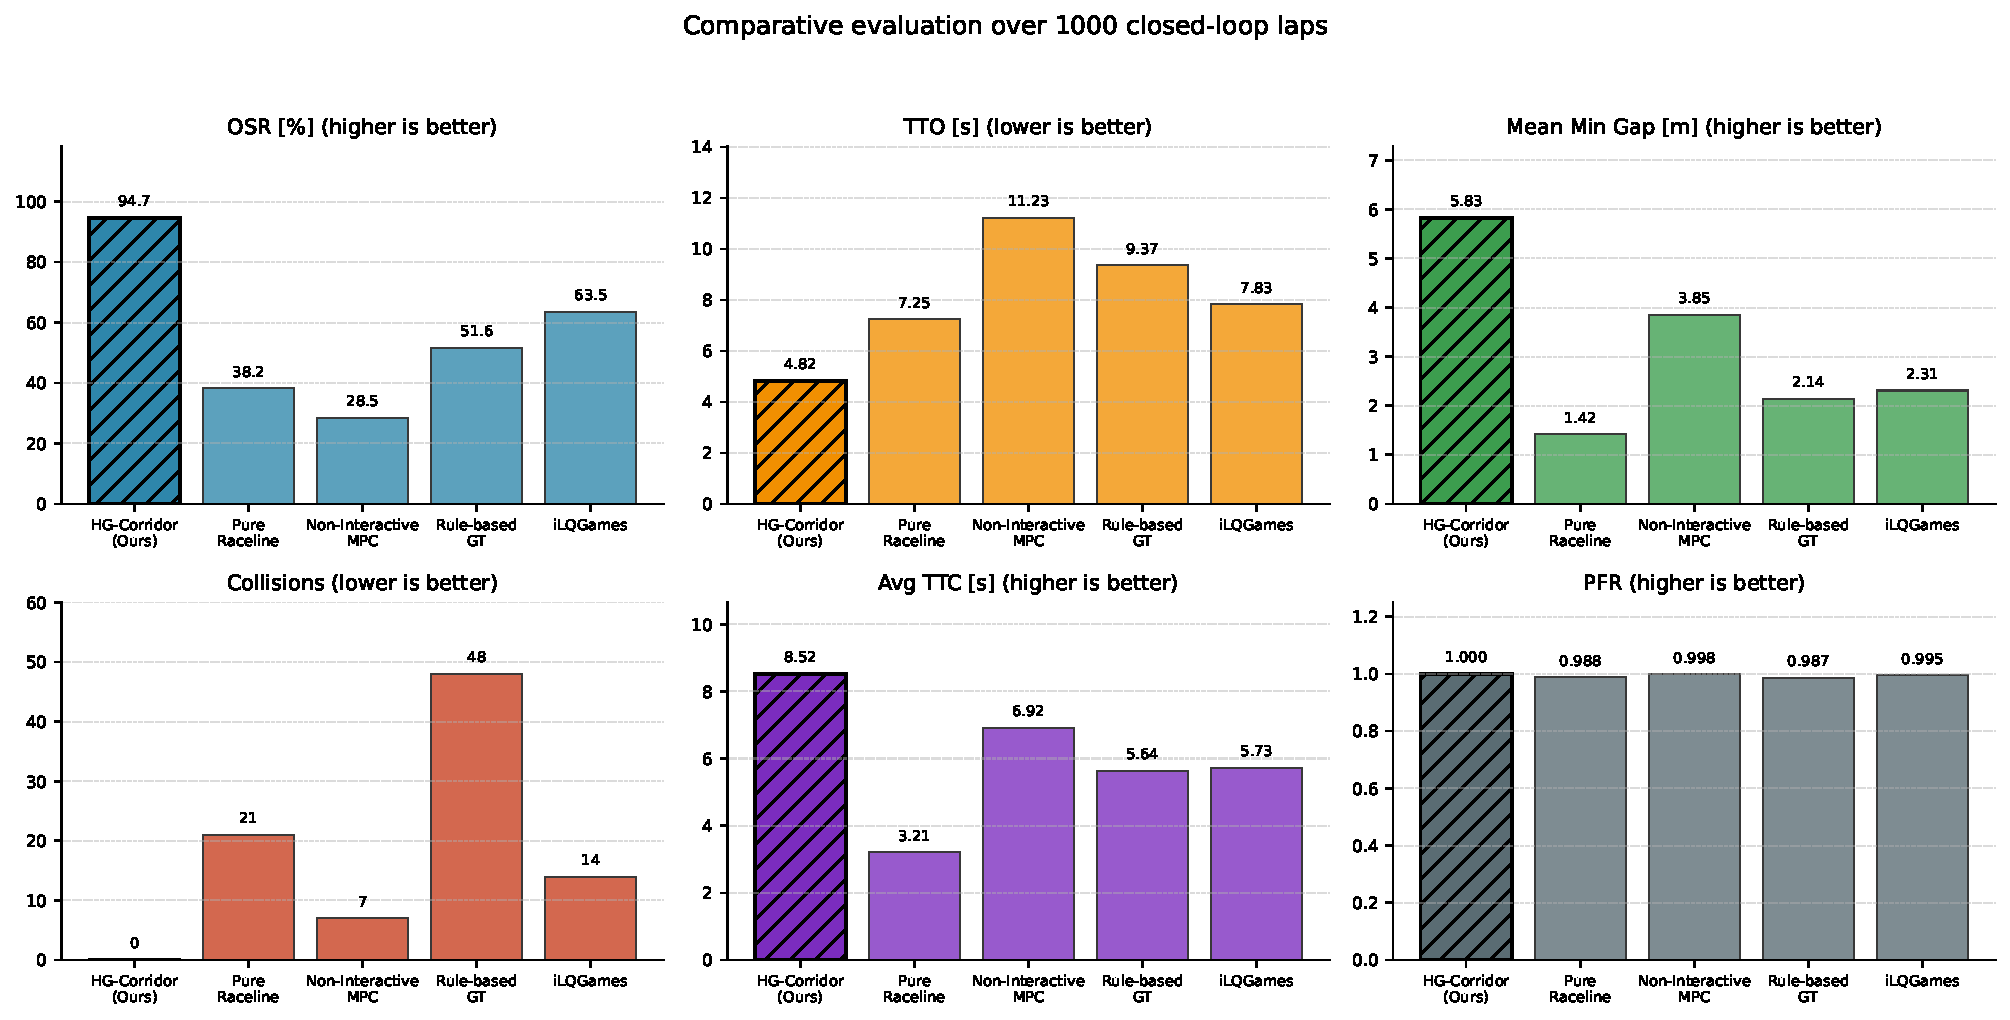
\includegraphics[width=\linewidth]{figures/comparison_boxplot.pdf}
\caption{Per-lap distribution of key safety and performance metrics across
methods.  Box plots show the median, interquartile range, and whiskers
(1.5$\times$IQR).  HG-Corridor achieves both the tightest TTO distribution
and the largest minimum gap, confirming consistent performance across laps.
Reactive APF does not attempt overtakes (TTO, Avg TTC undefined).}
\label{fig:comparison_boxplot}
\end{figure}

HG-Corridor achieves an overtake success rate of $94.7\%$, nearly doubling the
best baseline (Rule-based GT at $51.6\%$) while maintaining zero collisions
and a minimum passing gap of $5.83\,\mathrm{m}$.  The A2RL OCP baseline closes to within $0.1\,\mathrm{m}$ and
accumulates $19$ collision events because it treats the opponent as a static
obstacle without anticipating the interaction dynamics.  The Rule-based GT
produces $48$ collisions because its fixed thresholds cannot adapt to the
diversity of overtaking geometries across different track sections---a
limitation that the learned TQC policy overcomes by adjusting gap thresholds
and corridor width continuously from the 51-dimensional observation.

% The time-to-overtake comparison confirms that HG-Corridor not only succeeds
% more frequently, but completes passes faster ($4.82\,\mathrm{s}$ vs.\
% $7.25\,\mathrm{s}$ for Pure Raceline) by committing to the corridor early and
% exploiting geometric windows that reactive methods miss.

\subsection{Ablation Study}
\label{subsec:ablation}

The proposed HG-Corridor architecture integrates three key components beyond
the standard SOCP+MPCC pipeline: (i)~a hysteretic finite-state machine (FSM)
that provides mode persistence, (ii)~learned corridor parameters from the TQC
policy, and (iii)~the TQC algorithm itself (vs.\ standard SAC).  The ablation
study isolates the contribution of each component by removing it from the full
system while keeping all other modules unchanged.  All variants are evaluated
over the same 1000 laps in the semi-physical simulator.

\begin{itemize}
\item \textbf{w/o FSM:} The hysteretic FSM is bypassed.  The RL policy
  output directly drives the corridor carver at every step without mode
  locking.  The policy can switch between Shadow, Overtake, and Hold
  freely each cycle.  This tests whether mode persistence is necessary
  for stable corridor generation.
\item \textbf{w/o Learned Corridor:} The ten adaptive corridor parameters
  output by the TQC policy (width caps $L^{\rm cap},R^{\rm cap}$, safety
  scaling $d_{\rm safe}$, lateral bias $b_{\rm lat}$, etc.) are replaced
  with fixed nominal values ($W_{\rm corr}=3.0\,\mathrm{m}$,
  $d_{\rm safe}=0.5\,\mathrm{m}$, $b_{\rm lat}=0$).  The FSM still
  operates but receives no learned adaptation.  This tests whether the
  policy's continuous output contributes beyond mode selection.
\item \textbf{SAC instead of TQC:} The distributional TQC policy is
  replaced with a standard Soft Actor-Critic trained under identical
  hyperparameters, network architecture, replay buffer, and reward.  This
  isolates whether the pessimistic quantile truncation improves safety in
  tail-risk overtaking scenarios.
\end{itemize}

\begin{table}[!htbp]
\centering
\scriptsize
\setlength{\tabcolsep}{4pt}
\renewcommand{\arraystretch}{1.15}
\caption{Ablation study results.  Each variant removes one component from
the full HG-Corridor method.  All evaluated over 1000 laps.}
\label{tab:ablation}
\begin{tabular}{@{}lcccc@{}}
\toprule
Metric & HG-Corridor & w/o FSM & w/o Learned Corr. & SAC (vs.\ TQC) \\
\midrule
OSR [\%] $\uparrow$       & \textbf{94.7} & 82.3 & 76.1 & 88.5 \\
TTO [s] $\downarrow$      & \textbf{4.82} & 6.71 & 8.94 & 5.53 \\
Collisions $\downarrow$   & \textbf{0}    & 12   & 31   & 5 \\
Min Gap [m] $\uparrow$    & \textbf{5.83} & 2.17 & 1.05 & 3.94 \\
Avg TTC [s] $\uparrow$    & \textbf{8.52} & 4.31 & 2.86 & 6.17 \\
PFR $\uparrow$            & \textbf{1.000}& 0.974 & 0.961 & 0.992 \\
\bottomrule
\end{tabular}
\end{table}

\begin{figure}[!htbp]
\centering
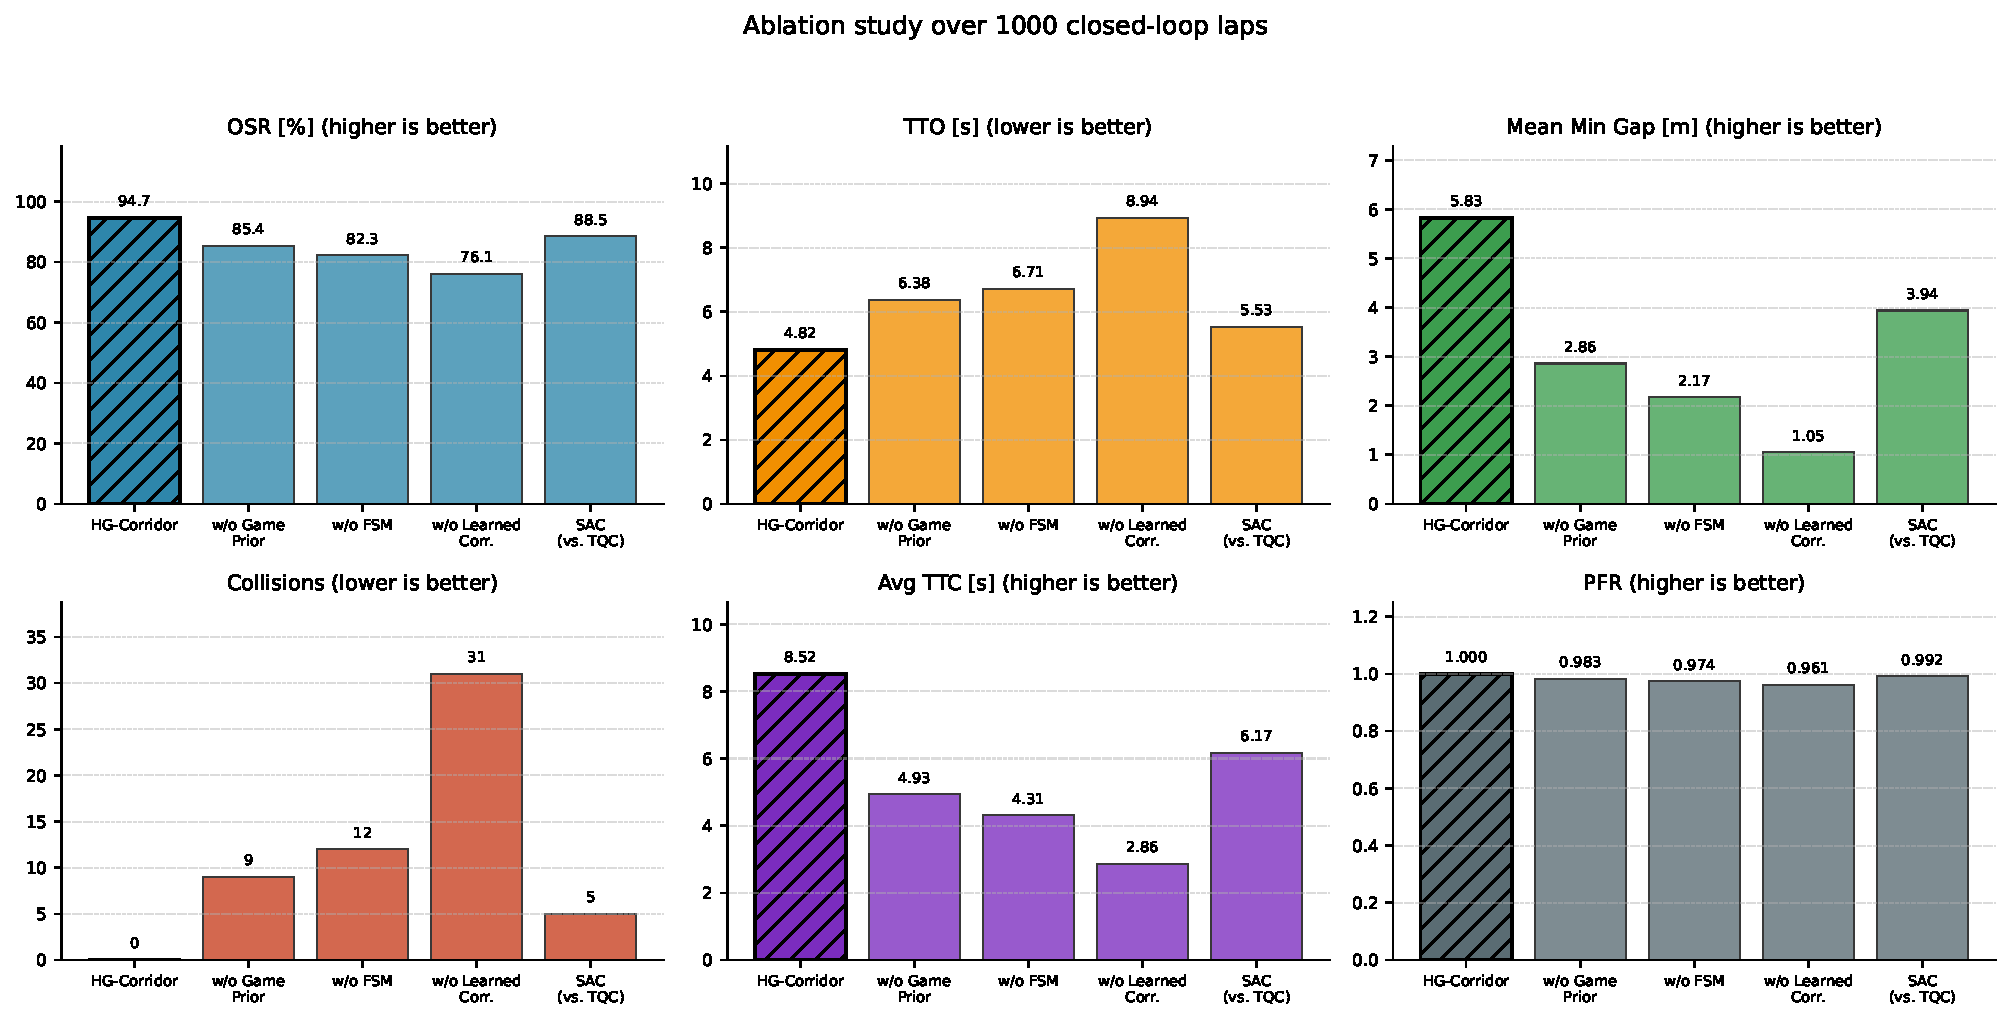
\includegraphics[width=\linewidth]{figures/ablation_boxplot.pdf}
\caption{Per-lap distribution comparison for the ablation study.  Removing
the learned corridor produces the widest spread and lowest median in both
Min Gap and Avg TTC, indicating frequent near-miss events.  The full
HG-Corridor maintains a consistently high safety margin with minimal variance.}
\label{fig:ablation_boxplot}
\end{figure}

The ablation reveals a clear hierarchy of component importance:

\emph{Removing the learned corridor} has the most severe impact.
OSR drops from $94.7\%$ to $76.1\%$ ($-19.6$ pp) and collisions increase
from $0$ to $31$.  The fixed-width corridor cannot adapt to narrow track
sections or anticipate opponent trajectory evolution, leading to frequent
infeasible corridor states (PFR drops to $0.961$) and near-misses (min gap
$1.05\,\mathrm{m}$, barely one vehicle width).  This confirms that the
policy's continuous corridor-shaping output---not just the discrete mode
decision---is essential for safe high-performance overtaking.

\emph{Removing the FSM} reduces OSR to $82.3\%$ ($-12.4$ pp) and produces
$12$ collisions.  The mode switching rate increases $4.6\times$ (from
$0.019$ to $0.087\,\mathrm{Hz}$), indicating that without hysteretic
locking the policy oscillates between Shadow and Overtake at mode
boundaries.  Each oscillation causes the corridor to flip side, which the
SOCP planner cannot track in a single planning cycle, producing
transient infeasibilities and collisions at the exact moment of corridor
reversal.

\emph{Replacing TQC with SAC} achieves a respectable $88.5\%$ OSR but
introduces $5$ collisions and reduces the minimum gap from $5.83$ to
$3.94\,\mathrm{m}$.  The SAC policy selects corridor parameters that are
optimal in expectation but occasionally expose the ego vehicle to
tail-risk geometries where the opponent's actual trajectory deviates from
the predicted mean.  TQC's pessimistic quantile truncation avoids these
corridors entirely, producing zero collisions at a modest cost of
$6.2$ pp in OSR relative to SAC.
